\chapter{宇宙学}\label{chpt:cosmology}

现在将我们对流形的野心施以整个宇宙上。
观测结果建议，宇宙在大尺度上\textbf{空间均匀}(homogeneous)且\textbf{各向同性}(isotropic)，即空间平移对称和旋转对称。
这使得不能用非零质量密度和常数场强求解 Poisson 方程，因为试图计算某点场强时，要涉及对充斥全空间的物质做积分，这是反常积分，需用有限域逼近。简单计算就可发现结果“为零”或“发散”，取决于趋于无穷的方式，说明积分不良定义，则称为\textbf{Neumann-Zeeliger 疑难}。可见 Newton 引力论很难发展出宇宙学。
宇宙学的早期发展毫无疑问是 Einstein 带头，广义相对论可以自然地研究均匀各向同性的解及其扰动。

\section{运动学}\label{sec:cosmo-kinematics}

\subsection{宇宙学原理}

我们怎样从星系的位置和到达地球的星光推断宇宙的几何？\footnote{本章的几何、动力学与热史据梁灿彬、周彬《微分几何入门与广义相对论》上册第二版第 10 章（科学出版社，2006 年，第 358--418 页）组织。观测值的出处另注。}局域引力实验可以重复，宇宙的演化史却只有一部。要从今天的观测追溯过去，须先说明在哪个尺度上描述物质。星系聚成星系群、星系团，团与团之间又有大片空洞。若在数亿光年的尺度上取平均，取样体积已包含许多星系团，这时才可问平均密度是否还随位置改变。\textbf{宇宙学原理}(cosmological principle) 假设，在足够大的尺度上，每一时刻的宇宙空间均匀且各向同性。具体说，存在一族充满时空的\textbf{共动观者}，对每位观者，大尺度物质分布没有优先方向，同一时刻各处的平均密度、压强等标量也相同。这里及下文的星系均指随平均物质运动的星系，其本动须另作修正。在恒星或星系近旁，局域引力场必须另求，例如孤立球形星体的外部解见第~\ref{chpt:BH}~章。我们只能从自己的世界线接收信号，故在一处见到天空各向同性，还须假设我们所处的位置没有特殊性，才能把这一性质推广到各处。

这里的“同时”须加以确定。将时空分成一族类空超曲面 $\Sigma_s$，使每一事件恰在其中一面上。\textbf{空间均匀}要求同一面上任意两点可由保持空间度规及物质分布的对称变换互换；每一面称\textbf{均匀面}。\textbf{各向同性}则是对观者而言的。设 $U^\mu$ 是观者在 $p$ 点的 4-速，对任意两个与 $U^\mu$ 正交的等长矢量，总有保持 $p$ 和 $U^\mu$ 的时空等度规变换，把一个矢量映到另一个，物质分布也随之不变。

通常物质选定了一族均匀面。例如平均密度随时间单调变化时，等密度面便标出了这一族面。若均匀面族唯一，则过 $p$ 的均匀面在上述旋转下保持不变，其单位法矢在观者静止空间的投影也须不变。任意空间旋转都保留的矢量只有零矢量，故 $U^\mu$ 正交于均匀面。唯一性的条件不能略去，例如在闵氏真空中，每个惯性系都有自己的一族均匀面。以下采用宇宙物质所定的均匀面和正交于它的\textbf{宇宙静系}。

\subsection{均匀面的几何}

记 $h_{ij}$ 为均匀面上的诱导度规。要判断这张三维空间有几种可能的几何，只须考察过一点的截面曲率。由 \S\ref{sec:curvature} 的曲率张量对称性，曲率可看成作用在 2-形式上的对称算子。三维中取 Hodge 对偶即把单位 2-形式化为单位法矢；转动法矢便可把任一平面转到另一平面。因此各截面的曲率都取同一值 $K$，空间均匀性又使 $K$ 在该面上处处相等。于是
\begin{equation}\label{eq:cosmo-space-curvature}
    {}^{(3)}\!R_{ijkl}=K(h_{ik}h_{jl}-h_{il}h_{jk}),\qquad
    {}^{(3)}\!R_{ij}=2Kh_{ij},\qquad {}^{(3)}\!R=6K .
\end{equation}
事实上，一旦有了第一式，连通的三维空间中便不再需要另用均匀性。将后两式代入缩并 Bianchi 恒等式 \eqref{eq:Bianchi} 的三维形式，即有 $2\p_j K=3\p_j K$。各时刻的 $K$ 仍可不同。

三维常曲率空间有六个独立的局部 Killing 场：三个可移走所选的点，另三个固定该点而转动标架。其局部几何由 $K$ 完全决定，因而为每个 $K$ 构造一个例子就够了。$K=0$ 时取欧氏空间，以距原点的距离为径向坐标。$K>0$ 时取四维欧氏空间中的球面 $W^2+\bm X^2=b^2$，令 $W=b\cos\chi$，$\bm X=b\sin\chi\,\bm n$，其中 $\bm n$ 是三维单位矢量。由 $\bm n\cdot\d\bm n=0$ 和 $\d\bm n^2=\d\Omega^2$，球面上的线元为 $b^2(\d\chi^2+\sin^2\chi\,\d\Omega^2)$。类似地，在辅助闵氏空间中取双曲面的上叶 $W^2-\bm X^2=b^2$，令 $W=b\cosh\chi$，$\bm X=b\sinh\chi\,\bm n$。代入 $-\d W^2+\d\bm X^2$ 就得正定线元 $b^2(\d\chi^2+\sinh^2\chi\,\d\Omega^2)$。两个曲面上的单位法矢都是位置矢量除以 $b$，故第二基本形式为 $\pm h_{ij}/b$，符号取决于法向及外曲率惯例。平直背景的 Gauss 方程给出式 \eqref{eq:cosmo-space-curvature}，球面的法矢类空，$K=1/b^2$，双曲面的法矢类时，$K=-1/b^2$。

常曲率只决定局部几何。通常取完备单连通的空间，三种可能便是 $S^3,\mathbb E^3,H^3$。球面有限而无边界，后两者的体积无限。若放弃单连通性，还可把等价点按离散等度规变换作粘合。例如将平直空间的三个坐标各自周期化，就得体积有限的平直三维环面。这样的粘合保留局部曲率，却可能破坏全局各向同性。

\subsection{Robertson--Walker 度规}

在一张均匀面上给星系编上坐标 $x^i$，沿各自的世界线保持 $x^i$ 不变，便得\textbf{共动坐标}。按 \S\ref{sec:sync-clock} 的对钟条件，先以均匀面的标号 $\lambda$ 为时间，正交性使线元形如 $-N^2\d\lambda^2+h_{ij}\d x^i\d x^j$。共动观者的 4-加速度与 $U^\mu$ 正交，各向同性要求这个空间矢量为零。在上述正交坐标中，其空间分量为 $\p_i\ln N$，故 $N$ 只随 $\lambda$ 而变。取 $\d t=N(\lambda)\d\lambda$ 并在同一均匀面上对准所有钟的零点，便得到\textbf{宇宙时} $t$。它是每一共动观者的固有时，此系中 $U=\p_t$，$g_{00}=-1$，$g_{0i}=0$。相应地，式 \eqref{eq:metric-christ} 给出 $\Gamma^\mu_{00}=0$，故 $x^i$ 恒定的曲线就是这族测地线。

两邻近星系间的尺长如何随时间变？在共动坐标下，按 \S\ref{sec:timelike}，形变由 $\tfrac12\p_t h_{ij}$ 给出。各向同性使这一对称张量只能正比于 $h_{ij}$，均匀性又使比例系数 $H$ 仅依赖 $t$。积分 $\p_t h_{ij}=2Hh_{ij}$ 得 $h_{ij}(t,x)=a^2(t)\gamma_{ij}(x)$，其中 $a>0$，$H=\dot a/a$，点表示对宇宙时求导。因而在任意两时刻，沿任意方向的尺长都按同一比例变化，$a$ 称\textbf{尺度因子}(scale factor)。将 $\gamma_{ij}$ 的常曲率归一为 $k=+1,0,-1$，依次记 $S_k(\chi)=\sin\chi,\chi,\sinh\chi$，则
\begin{equation}\label{eq:cosmo-rw}
    \d s^2=-\d t^2+a^2(t)\left[\d\chi^2+S_k^2(\chi)\d\Omega^2\right],
    \qquad \d\Omega^2=\d\theta^2+\sin^2\theta\,\d\varphi^2 .
\end{equation}
这是\textbf{Robertson--Walker 度规}，也称 Friedmann--Lemaître--Robertson--Walker（FLRW）度规。宇宙学原理只确定了线元的形式；还须由引力场方程和宇宙的物质含量确定 $a(t)$。每张均匀面的截面曲率为 $K(t)=k/a^2(t)$。特别是 $k=0$ 只说明三维空间平直，四维时空仍可弯曲。

径向固有距离在同一均匀面上量取。以共动星系 $A$ 为原点，$B$ 的径向坐标为 $\chi$，则 $D_{AB}(t)=a(t)\chi$。以 $A$ 为心过 $B$ 的二球面面积却是 $4\pi a^2 S_k^2(\chi)$。若取 $r=S_k(\chi)$，由 $(S'_k)^2=1-k S_k^2$ 可将式 \eqref{eq:cosmo-rw} 中的方括号改写为 $\d r^2/(1-kr^2)+r^2\d\Omega^2$；$k=+1$ 时 $r=\sin\chi$ 只能单调地覆盖一个半球。$k=\pm1$ 时 $a$ 就是曲率半径，有长度量纲；$k=0$ 时常数倍的归一化可吸收进共动坐标。体元为 $a^3 S_k^2(\chi)\sin\theta\,\d\chi\,\d\theta\,\d\varphi$。对整个 $S^3$，两极对应 $\chi=0,\pi$，故 $V=4\pi a^3\int_0^\pi\sin^2\chi\,\d\chi=2\pi^2a^3$。

最后看光锥。引入\textbf{共形时} $\d\eta=\d t/a$ 后，径向光线有 $\d\chi=\pm\d\eta$，第 \ref{chpt:BH} 章用此式讨论过宇宙学视界。$k=0$ 时一眼即见时空共形平直，其余两种也可直接验证。令 $u=\eta-\chi$，$v=\eta+\chi$，再取 $T-R=f(u)$，$T+R=f(v)$。若 $k=-1$ 取 $f(x)=\e^x$，若 $k=+1$ 取 $f(x)=\tan(x/2)$。在坐标正则处，两种选取都满足 $R^2=f'(u)f'(v)S_k^2(\chi)$，于是
\[
    \d s^2=\frac{a^2}{f'(u)f'(v)}
    \big[-\d T^2+\d R^2+R^2\d\Omega^2\big].
\]
这里的共形因子一般随时空点改变，故共形平直与时空曲率消失是两件事。

\section{动力学}\label{sec:cosmo-dynamics}

\subsection{星系的退行与红移}

Slipher 测过 41 个河外星系的光谱，其中 36 个的谱线向长波方向移动。Hubble 又测量星系距离，于 1929 年指出，近邻星系的红移随距离近似线性增长。测红移只须比较同一谱线的观测波长与实验室波长，距离却要另找标尺。星系本身的运动也会使谱线移动，近邻中甚至有蓝移的例子。

在共动星系间的固有距离 $D=a\chi$ 中，$\chi$ 不随时间变，故对时间求导便得\textbf{Hubble 定律} $v_{\rm rec}(t):=\dot D(t)=H(t)D(t)$。其中 $H(t)$ 称\textbf{Hubble 参数}。下标 $0$ 表示今天，$H_0=H(t_0)$ 称\textbf{Hubble 常数}。$H_0>0$ 时，每个共动星系都看到其余星系退行，均匀膨胀没有中心。$D>H^{-1}$ 时 $\dot D>1$，因为此处求导比较的是两张同时面上端点间的距离。共动星系经过某一局域观者时，这位观者所测的相对速率仍小于光速。

观测在过去光锥上进行。设共动星系于 $t_{\rm e}$ 发光，共动观者于 $t_{\rm o}$ 接收。沿用第~\ref{chpt:BH}~章引力红移的频率定义，未来指向的光波矢 $K^\mu$ 给出 $\omega=-U_\mu K^\mu=K^t$。取仿射参数 $\beta$，由 $K^\nu\cd_\nu K^\mu=0$ 和 $\cd_\mu U_\nu=H(g_{\mu\nu}+U_\mu U_\nu)$，有
\begin{equation}\label{eq:cosmo-redshift}
    \frac{\d\omega}{\d\beta}
    =-K^\mu K^\nu\cd_\mu U_\nu=-H\omega^2,
    \qquad
    1+z:=\frac{\lambda_{\rm o}}{\lambda_{\rm e}}
    =\frac{\omega_{\rm e}}{\omega_{\rm o}}
    =\frac{a(t_{\rm o})}{a(t_{\rm e})}.
\end{equation}
其中 $\lambda_{\rm e},\lambda_{\rm o}$ 是两端测得的波长，积分用到了 $\d t/\d\beta=\omega$。也可把坐标原点置于光源，使光线为径向。相邻波峰走过相同的共动距离 $\int_{t_{\rm e}}^{t_{\rm o}}\d t/a(t)$，故两端周期之比正好等于尺度因子之比。膨胀时光子逐渐红移，收缩时则蓝移。近源满足 $t_{\rm o}-t_{\rm e}\simeq D_0$，将 $a$ 展开至一阶便得观测关系 $z\simeq H_0D_0$。在这一精度内 $z$ 也等于低速 Doppler 退行速率；对远源则应使用式 \eqref{eq:cosmo-redshift}。

\subsection{尺度因子的演化}

Friedmann 于 1922 年求得随时间演化的正曲率解，Einstein 于次年撤回了对其计算的异议。在星系无规速率可忽略的尺度上，星系的质量分布可看作\textbf{尘埃}，压强 $p_{\rm m}\simeq0$。各向同性的超相对论粒子构成\textbf{辐射}，其能动张量迹为零，故 $p_{\rm r}=\rho_{\rm r}/3$。沿用第 1 章“流体力学”的理想流体能动张量，以 $\rho$ 表示该节的共动能量密度 $\varepsilon$。在此共动系中，非零分量为 $T_{00}=\rho(t)$、$T_{ij}=p(t)g_{ij}$，此处 $\rho,p$ 均不含单列的 $\Lambda$ 项，仍用几何单位 $G=c=1$。由式 \eqref{eq:cosmo-rw}，混合时空分量 $G_{0i}=0$，其余分量为 $G_{00}=3(H^2+k/a^2)$ 和 $G_{ij}=-(2\ddot a/a+H^2+k/a^2)g_{ij}$。代入 \S\ref{sec:Einstein} 的场方程便得
\begin{equation}\label{eq:cosmo-friedmann}
    H^2=\frac{8\pi}{3}\rho-\frac{k}{a^2}+\frac{\Lambda}{3},
    \qquad
    \frac{\ddot a}{a}=-\frac{4\pi}{3}(\rho+3p)+\frac{\Lambda}{3}.
\end{equation}
第一式称\textbf{Friedmann 方程}。第二式中压强与密度一道影响加速度。对第一式求导，再用第二式消去 $\ddot a$，得能量方程 $\dot\rho+3H(\rho+p)=0$，亦可直接从 $\cd_\mu T^{\mu\nu}=0$ 得到。它在共动体积 $V\propto a^3$ 内可写成 $\d(\rho V)=-p\,\d V$。给定状态方程，在 $\dot a\ne0$ 的区间只须独立求解 Friedmann 方程与能量方程，在转折处可用加速度方程续解。

若某一组分单独守恒且 $p=w\rho$，其中 $w$ 为常数，则 $\rho\propto a^{-3(1+w)}$。故尘埃有 $\rho_{\rm m}a^3=\text{常数}$，辐射有 $\rho_{\rm r}a^4=\text{常数}$。前者只是共动体积中的质量不变，后者除了粒子数密度随体积稀释，每个自由光子的能量还随 $a^{-1}$ 减小。因此向过去追溯，辐射与尘埃的密度比按 $a^{-1}$ 增长。

先置 $\Lambda=0$。有普通物质或辐射时，$\rho>0$、$p\geqslant0$ 给出 $\ddot a<0$。从当今的膨胀支向过去回溯，斜率至少为 $\dot a_0>0$，故 $a$ 在有限固有时以前就降至零，取该端点为 $t=0$。任意固定共动间隔的固有长度都趋零，空间各处的密度一道发散。这就是该模型的\textbf{大爆炸奇性}(big bang singularity)。共动测地线向过去不完备；较弱假设下的不完备性见 \S\ref{sec:Hawking}。这里 $a\to0$ 是同一对共动点间距离的极限，对于非紧的平直或双曲切片，每一 $t>0$ 的空间仍可无限延伸。

对纯辐射取常数 $B=(8\pi\rho_{\rm r}a^4/3)^{1/2}>0$。以 $a^2$ 为未知量，初始膨胀支满足 $\d(a^2)/\d t=2\sqrt{B^2-ka^2}$。取 $a(0)=0$，得
\begin{equation}\label{eq:cosmo-radiation}
    \dot a^2=\frac{B^2}{a^2}-k,\qquad a^2(t)=2Bt-kt^2 .
\end{equation}
三支在初期均有 $a\simeq\sqrt{2Bt}$。$k=+1$ 的解在 $t=B$ 达到 $a=B$，又于 $t=2B$ 缩回零。$k=0$ 的解按 $t^{1/2}$ 膨胀，$k=-1$ 的解在晚期趋于匀速膨胀。

对纯尘埃取常数 $A=8\pi\rho_{\rm m}a^3/3>0$，故 $\dot a^2=A/a-k$。以共形时 $\d\eta=\d t/a$ 作参数，上式成为 $(\d a/\d\eta)^2=Aa-ka^2$。取 $a(0)=0$，得到
\begin{equation}\label{eq:cosmo-dust}
    \begin{array}{c|cc}
       k & a(\eta) & t(\eta) \\ \hline
       +1 & A(1-\cos\eta)/2 & A(\eta-\sin\eta)/2 \\
        0 & A\eta^2/4 & A\eta^3/12 \\
       -1 & A(\cosh\eta-1)/2 & A(\sinh\eta-\eta)/2
    \end{array}
\end{equation}
其中闭支取 $0<\eta<2\pi$，其余两支取 $\eta>0$。$k=0$ 给出 $a=(9A/4)^{1/3}t^{2/3}$，也是三支的早期渐近式。闭支于 $\eta=\pi$ 膨胀至 $a=A$ 后回缩，其收缩段正给出第~\ref{chpt:BH}~章 Oppenheimer--Snyder 尘埃球的内部解。

\begin{figure}[htbp]
    \centering
    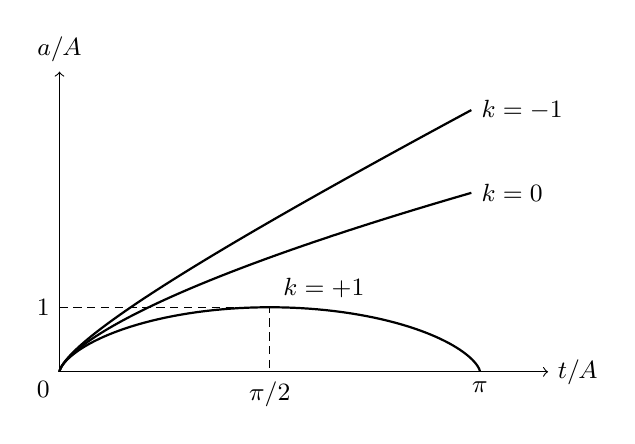
\begin{tikzpicture}[x=1.7cm,y=.82cm, font=\small]
        \draw[->] (0,0) -- (3.65,0) node[right] {$t/A$};
        \draw[->] (0,0) -- (0,4.65) node[above] {$a/A$};
        \draw[thick,domain=0:6.283185,samples=96,variable=\u]
            plot ({(\u-sin(deg(\u)))/2},{(1-cos(deg(\u)))/2});
        \draw[thick,domain=0:3.33,samples=64,variable=\u]
            plot ({\u^3/12},{\u^2/4}) node[right] {$k=0$};
        \draw[thick,domain=0:2.90,samples=64,variable=\u]
            plot ({(sinh(\u)-\u)/2},{(cosh(\u)-1)/2}) node[right] {$k=-1$};
        \draw[densely dashed] (0,1) node[left] {$1$} -- (1.5708,1) -- (1.5708,0) node[below] {$\pi/2$};
        \node[above right] at (1.6,1) {$k=+1$};
        \node[below] at (3.14159,0) {$\pi$};
        \node[below left] at (0,0) {$0$};
    \end{tikzpicture}
    \caption{相同尘埃常数 $A$、$\Lambda=0$ 的三种宇宙。$a\ll A$ 时曲率项在 $\dot a^2=A/a-k$ 中可忽略，故三支从相同的幂律分开。}
    \label{fig:cosmo-dust}
\end{figure}

尘埃与辐射并存时，也可不求显式解而判断宇宙的命运。由能量守恒有 $\d(\rho a^3)/\d a=-3pa^2\leqslant0$。因此随 $a$ 增大，$8\pi\rho a^2/3$ 至少按 $a^{-1}$ 衰减。若 $k=0$ 或 $-1$，膨胀支的 $\dot a$ 始终为正，晚期分别趋于 $0$ 和 $1$。若 $k=+1$，上述衰减项在有限 $a_{\max}$ 降至 $1$，这时 $\dot a=0$。因 $\rho(a_{\max})>0$，加速度在此仍严格为负，故转折发生在有限时刻，继而收缩至\textbf{大挤压}(big crunch)。这一按空间曲率分类的结论用到了 $\Lambda=0$ 和普通物质的压强条件。

\subsection{膨胀年龄与静态解}

匀速倒推至 $a=0$ 所需时间为 $a_0/\dot a_0=H_0^{-1}$，称\textbf{Hubble 时间}。若整个膨胀期均有 $\ddot a<0$，则 $a(t)$ 在当今切线之下，年龄 $t_0<H_0^{-1}$。若曾有加速膨胀，这个上界就须重新检验。实用单位常记 $H_0=100h\,\mathrm{km\,s^{-1}\,Mpc^{-1}}$，其中 $1\,\mathrm{Mpc}=10^6\,\mathrm{pc}$，$1\,\mathrm{pc}\simeq3.26$ 光年，故 $H_0^{-1}\simeq9.78h^{-1}\,\mathrm{Gyr}$。早期的距离标定使 Hubble 高估了 $H_0$，由此推得的年龄甚至短于地球的放射性定年。修订距离标尺后，这一矛盾消解。

如今两种测法对 $H_0$ 仍给出不同的结果，以下均以 $\mathrm{km\,s^{-1}\,Mpc^{-1}}$ 为单位。Planck 用微波背景的温度、偏振和引力透镜数据，在平直的冷暗物质与宇宙学常数模型中推得 $H_0=67.4\pm0.5$。SH0ES 用几何距离标定造父变星，再标定 Ia 型超新星，由近邻宇宙的距离与红移测得 $73.04\pm1.04$。2026 年 H0DN 联合多种局域距离标尺，得 $73.50\pm0.81$。早期宇宙的模型推断与局域距离标定之间的差异称为\textbf{Hubble 张力}。\footnote{\href{https://doi.org/10.1051/0004-6361/201833910}{Planck Collaboration（2020）}，\href{https://doi.org/10.3847/2041-8213/ac5c5b}{Riess 等（2022）}，\href{https://doi.org/10.1051/0004-6361/202557993}{H0DN Collaboration（2026）}。}

对 $\Lambda=0$ 的纯尘埃宇宙，还可给出膨胀至任意尺度的年龄。记 $x=a/a_0$，以\textbf{临界密度} $\rho_{\rm c0}=3H_0^2/(8\pi)$ 定义 $\Omega_0=\rho_{\rm m0}/\rho_{\rm c0}$。则 $k/a_0^2=H_0^2(\Omega_0-1)$。由式 \eqref{eq:cosmo-dust} 消去 $A$，得膨胀支的年龄函数
\[
    H_0 t(x)=
    \begin{cases}
        \dfrac{\Omega_0(\eta-\sin\eta)}{2(\Omega_0-1)^{3/2}},
        & \Omega_0>1,\quad
          \sin^2(\eta/2)=(1-\Omega_0^{-1})x,\\[5pt]
        \dfrac23 x^{3/2}, & \Omega_0=1,\\[5pt]
        \dfrac{\Omega_0(\sinh\eta-\eta)}{2(1-\Omega_0)^{3/2}},
        & 0<\Omega_0<1,\quad
          \sinh^2(\eta/2)=(\Omega_0^{-1}-1)x .
    \end{cases}
\]
其中闭支取 $0\leqslant\eta\leqslant\pi$。当今年龄取 $x=1$，闭、开两支分别代入 $\eta_0=2\arcsin\sqrt{1-1/\Omega_0}$、$\eta_0=2\operatorname{arsinh}\sqrt{1/\Omega_0-1}$ 即得 $t_0$。平直情形尤为简单，$t_0=2/(3H_0)$；闭支的收缩阶段则取同一 $x$ 对应的另一角 $2\pi-\eta$。

还有一种检验只须给宇宙年龄设下限。银河系贫金属球状星团的色星等图给出其中老年星族的平均年龄 $t_{\rm GC}=(13.61\pm0.25\pm0.23)\,\mathrm{Gyr}$，两项误差分别来自统计和系统效应。\footnote{\href{https://arxiv.org/abs/2603.04872}{Valcin 等（2026）}。} 宇宙在星团形成时已有一段历史，故须有 $t_0>t_{\rm GC}$。即使取较低的 $H_0=67.4\,\mathrm{km\,s^{-1}\,Mpc^{-1}}$，纯尘埃平直解也只给 $t_0\simeq9.7\,\mathrm{Gyr}$，容不下这批老星。由同一 Planck 数据拟合的含 $\Lambda$ 平直模型则给出约 $13.8\,\mathrm{Gyr}$。

最后问宇宙能否保持静止。尘埃有 $\rho_{\rm m}>0$，在 $\Lambda=0$ 时总有 $\ddot a<0$。若保留 \S\ref{sec:Einstein} 的宇宙学常数，令式 \eqref{eq:cosmo-friedmann} 同时满足 $\dot a=\ddot a=0$，便得 $\Lambda=4\pi\rho_{\rm m}$、$k/a_{\rm E}^2=\Lambda$。因此给定密度后只能取 $k=+1$，静态半径为 $a_{\rm E}=\Lambda^{-1/2}$，这就是\textbf{Einstein 静态宇宙}。正 $\Lambda$ 的斥力恰与尘埃的引力平衡。若令 $a=a_{\rm E}(1+\delta)$，尘埃密度按 $(1+\delta)^{-3}$ 变化，加速度方程在线性阶给出 $\ddot\delta=\Lambda\delta$，故这一平衡对均匀尺度扰动不稳定。即使抽去尘埃，$\Lambda\ne0$ 仍要求真空满足 $R_{\mu\nu}=\Lambda g_{\mu\nu}$（第~\ref{chpt:BH}~章），从而排除了平直时空。特别地，式 \eqref{eq:dS-flat-slicing} 的空间截面平直，而四维曲率仍非零。

\section{热力学}\label{sec:cosmo-thermal}

\subsection{膨胀中的热平衡}

怎样给早期宇宙的钟标上温度？上一节从能量守恒得到了 $\rho_{\rm r}\propto a^{-4}$，只须再知道同一能量密度对应的温度。在热平衡下，暂取 $\hbar=c=k_{\rm B}=1$，有 $\rho_{\rm r}=(\pi^2/30)g_*T^4$。这里 $g_*$ 计入当时仍为相对论性的粒子自由度，同温的费米子每一自由度只按玻色子的 $7/8$ 计。$g_*$ 不变时有 $aT=\text{常数}$。若有粒子湮灭并把熵交给尚未退耦的热浴，应用共动熵守恒，即 $g_{*s}(aT)^3=\text{常数}$，其中 $g_{*s}$ 为熵的有效自由度数。

以大爆炸为时间零点。辐射为主时 $a\propto t^{1/2}$，曲率可忽略时 Friedmann 方程给出 $H=1/(2t)$。结合辐射的能量密度，得 $t\propto g_*^{-1/2}T^{-2}$；在秒和开尔文单位下，一秒左右的粗估是 $T\sim10^{10}\,{\rm K}\,(t/{\rm s})^{-1/2}$。同温下能参与热平衡的粒子种类越多，膨胀越快，宇宙的年龄越小。

能沿这条温度曲线一直走到 $t=0$ 吗？在上述平直辐射解中 $a\to0$，辐射的能动张量无迹，取 $\Lambda=0$ 竟有 $R=0$。但另一不变量 $R_{\mu\nu}R^{\mu\nu}=(8\pi)^2(\rho^2+3p^2)=3/(4t^4)$ 确实发散。恢复国际单位后，此式的末项为 $3/[4(ct)^4]$。在 Planck 时间 $t_{\rm P}=\sqrt{\hbar G/c^5}\simeq5.4\times10^{-44}\,{\rm s}$，曲率平方已达 $\ell_{\rm P}^{-4}$ 量级，$\ell_{\rm P}=ct_{\rm P}$。这是估计经典引力适用范围的尺度。\S\ref{sec:Hawking} 给出了过去类时测地不完备的充分条件；定理与上述具体解都不能给出 Planck 时期的物态，参见 \S\ref{sec:quantum-gravity}。

温度极高时，夸克、轻子、规范玻色子与它们的反粒子通过散射、产生和湮灭交换能量。设某种反应的每粒子速率为 $\Gamma=n\langle\sigma v\rangle$。若 $\Gamma\gg H$，一次显著膨胀之前足以发生许多次反应，粒子可维持局域热平衡。若 $\Gamma$ 降至 $H$ 以下，该反应来不及恢复平衡，相关粒子便\textbf{退耦}(decouple)或其丰度\textbf{冻结}(freeze out)。不同反应的截面各异，退耦也就有先后。粒子的静能若远小于 $k_{\rm B}T$，其典型动能足以使之作相对论性运动；反之，热浴中能产生粒子对的高能尾部受到指数压低。例如 $k_{\rm B}T\sim10\,{\rm MeV}$ 时 $\gamma+\gamma\leftrightarrow e^-+e^+$ 仍很快，核子与反核子的成对产生却已极罕见。

湮灭过后为何还有质子与中子？以 $\eta_{\rm b}=(n_{\rm b}-n_{\bar{\rm b}})/n_\gamma$ 量度\textbf{重子不对称性}。今天反重子稀少，每十亿个光子约对应一个重子。若正反重子起初略不等量，成对湮灭就会留下这个差额。若要从相等的初始丰度动态生成差额，通常须有破坏重子数守恒、破坏电荷共轭（$C$）及电荷共轭与空间反演的联合对称（$CP$）的过程，还须偏离热平衡。某些大统一模型的重粒子衰变可满足这些条件；究竟是哪一种过程留下了重子，仍须用观测辨别。

\subsection{从中微子退耦到原初核合成}\label{sec:cosmo-bbn}

$t\sim1\,{\rm s}$、$k_{\rm B}T\sim1\,{\rm MeV}$ 时，中微子的弱散射来不及追上膨胀。它们脱离电磁热浴，以后仍以能量密度参与引力。温度再降，正负电子的产生赶不上湮灭，大部分 $e^+e^-$ 对的熵转入光子。为使等离子体保持电中性，须留下与净正电荷等量的电子。取中微子瞬时退耦的近似，电磁热浴的 $g_{*s}$ 从 $2+(7/8)\times4=11/2$ 降至 $2$；退耦中微子的动量一直按 $a^{-1}$ 红移，故 $T_\nu/T_\gamma=(4/11)^{1/3}$。由此预期遗留至今的中微子背景温度近 $1.95\,{\rm K}$，这里的温度描述动量分布。

这批核子稍后能产生多少氦？高温下，$n+\nu_e\leftrightarrow p+e^-$、$n+e^+\leftrightarrow p+\bar\nu_e$ 维持中子与质子的化学平衡。因中子稍重，数密度比约为 $r_{\rm np}:=n_{\rm n}/n_{\rm p}\simeq\exp[-(m_{\rm n}-m_{\rm p})c^2/(k_{\rm B}T)]$。弱反应冻结后，自由中子仍会 $\beta$ 衰变。待核合成真正开始时，$r_{\rm np}$ 已降到约 $1/7$。

第一步是 $n+p\to{}^2{\rm H}+\gamma$。氘核虽有约 $2.22\,{\rm MeV}$ 的结合能，每个重子周围却有极多光子，能谱尾端仍足以打碎刚形成的氘。直到 $T$ 降至约 $10^9\,{\rm K}$、年龄达数分钟，才能越过这道\textbf{氘瓶颈}。氘俘获核子形成氚或 $^3{\rm He}$，再经 $^3{\rm H}+{}^2{\rm H}\to{}^4{\rm He}+n$ 或 $^3{\rm He}+{}^2{\rm H}\to{}^4{\rm He}+p$ 等反应形成 $^4{\rm He}$。几乎全部剩余中子进入氦核，每两个中子需另配两个质子，故氦的质量分数为 $Y_{\rm p}\simeq2r_{\rm np}/(1+r_{\rm np})\simeq1/4$。其余重子绝大部分留作氢。这个四分之一指重子质量的份额。

没有质量数为 $5$ 或 $8$ 的稳定核，密度又随膨胀迅速下降，反应链来不及大量合成重元素。残余氘和 $^3{\rm He}$ 相对于氢的核数比为 $10^{-5}$ 量级，质量数为 $7$ 的产物仅 $10^{-10}$ 量级，部分由 $^7{\rm Be}$ 衰变为 $^7{\rm Li}$。恒星内部有较高的密度和长得多的时间，可经三氦过程越过障碍。测原初丰度须选恒星加工较少的物质并校正其后演化。贫金属老星表面的锂丰度明显低于标准核合成按背景辐射所得重子密度预言的值，这一差异称为\textbf{原初锂问题}。

丰度还可反过来称量不可见的粒子。$\eta_{\rm b}$ 越大，氘越早越过瓶颈，也越易继续燃烧，残余氘对 $\eta_{\rm b}$ 尤为敏感。增加一族热平衡的轻中微子会提高同温时的 $\rho_{\rm r}$ 和 $H$，使中、质子互变在更高温度冻结，留下更多中子，因而提高 $Y_{\rm p}$。这使天文学能在加速器之外约束轻粒子种数。1977 年的氦丰度分析已能给轻中微子的种数设上限；如今这一方法约束的是核合成时相对论性组分的有效数 $N_{\rm eff}$，而 $Z$ 玻色子不可见衰变宽度独立给出约三种有标准弱耦合的轻中微子。

\subsection{最后散射与结构形成}\label{sec:cosmo-cmb}

辐射的能量密度比非相对论性物质多衰减一个 $a^{-1}$。因此先有物质与辐射密度相等，随后才有光子退耦，这两个时刻由不同条件决定。约在大爆炸后 $38$ 万年，$T\sim3000\,{\rm K}$，电子与原子核结合为中性原子，称为\textbf{复合}(recombination)。自由电子的骤减使 Thomson 散射率 $n_e\sigma_{\rm T}c$ 大幅下降。我们在各个方向收到的背景光子，大都在这段时期作最后一次散射；这些散射事件在过去光锥上形成有一定厚度的\textbf{最后散射面}。

退耦以后很少碰撞，光子为何仍能保持黑体谱？设 $\alpha=a/a_{\rm d}$，下标 $\rm d$ 指退耦。波长由 $\lambda_{\rm d}$ 变为 $\lambda=\alpha\lambda_{\rm d}$，单位体积中同一批光子的能量降至原来的 $\alpha^{-4}$。Planck 分布中的指数 $hc/(\lambda k_{\rm B}T)$ 在 $T=T_{\rm d}/\alpha$ 时恰保持不变。每单位波长的能谱密度于是满足
\[
   u_\lambda(\lambda,T)=\alpha^{-5}u_\lambda(\lambda/\alpha,T_{\rm d})
   =\frac{8\pi hc}{\lambda^5}\frac{1}{\exp[hc/(\lambda k_{\rm B}T)]-1}.
\]
故今天应见到一个几乎充满全天、峰值落在毫米波段的冷黑体，这就是\textbf{宇宙微波背景}(cosmic microwave background, CMB)。每单位频率和每单位波长的谱密度差着 Jacobian 因子，两种谱峰所对应的波长略有不同。

1965 年 Penzias 与 Wilson 在 $7.35\,{\rm cm}$ 波段测得几乎各向相同的额外天线温度，Dicke 等人随即将它解释为热大爆炸的遗迹。一个频点不能确定谱形。此后地面、气球及卫星测量覆盖了谱峰两侧，COBE 的 FIRAS 仪器测得接近 $2.725\,{\rm K}$ 的黑体谱。稳恒态宇宙很难产生这样的全天热背景。将温度图按球谐函数展开，扣除平均温度后，最强的是相对幅度约 $10^{-3}$ 的偶极。观者相对辐射静系以 $\bm v$ 运动，朝向 $\hat{\bm n}$ 的温差一阶为 $\Delta T/T\simeq\bm v\cdot\hat{\bm n}/c$，太阳系由此测得的速率约 $370\,{\rm km/s}$。扣除本动及银河前景，四极及更高多极留下约 $10^{-5}$ 量级的本征温度涨落，COBE 于 1992 年首次报告其大角尺度信号。\footnote{COBE 各仪器测量的物理量不同，可分别查阅 NASA 的 \href{https://lambda.gsfc.nasa.gov/product/cobe/about_firas.html}{FIRAS 光谱}和 \href{https://lambda.gsfc.nasa.gov/product/cobe/about_dmr.html}{DMR 全天温度图}。}

\begin{table}[htbp]
\centering\small
\caption{热大爆炸中的几个时标。$T$ 为光子温度；表中给的是量级，各过程均持续一段时间。}\label{tab:cosmo-thermal}
\begin{tabular}{@{}lll@{}}\toprule
宇宙年龄 & $T$ & 主要过程 \\ \midrule
$10^{-2}\,{\rm s}$ & $10^{11}\,{\rm K}$ & 光子、轻子热平衡，核子已很少 \\
$1\,{\rm s}$ & $10^{10}\,{\rm K}$ & 中微子退耦，中、质子互变冻结 \\
十余秒 & 数 $10^9\,{\rm K}$ & 大部分 $e^+e^-$ 对湮灭，加热光子 \\
数分钟 & $10^9\,{\rm K}$ 以下 & 氘得以保存，迅速合成氦 \\
约五万年 & 约 $10^4\,{\rm K}$ & 物质密度超过辐射密度 \\
约四十万年 & $3000\,{\rm K}$ & 氢复合，背景光子最后散射 \\
数亿年 & 数十 K & 首批恒星、星系逐渐形成 \\ \bottomrule
\end{tabular}
\end{table}

几乎均匀的宇宙怎样长出星系？令 $\delta=(\rho-\bar\rho)/\bar\rho$。在比 Hubble 半径小、引力弱且可用单一非相对论性流体描述的尺度上，波数为 $q$ 的共动 Fourier 模在线性近似中满足
\[
   \ddot\delta_q+2H\dot\delta_q+
   \left(\frac{c_s^2q^2}{a^2}-4\pi G\bar\rho\right)\delta_q=0 ,
\]
其中 $c_s$ 为绝热声速，$\bar\rho$ 为平均质量密度。压强支撑短波，引力放大长波，这给出 Jeans 判据。膨胀使增长放慢；在平直尘埃时期代入 $H=2/(3t)$ 即得增长模 $\delta\propto t^{2/3}\propto a$。Lifshitz 将膨胀背景上的扰动推广到相对论情形。复合前重子与光子紧耦合，光压使许多扰动作声振荡。若只有重子，从最后散射时的微小起伏很难及时长成所见星系。能提早聚集的冷暗物质先形成引力势阱，复合后的重子再向其中落入。

若暗物质在退耦时仍高速运动，自由飞行会抹平小尺度的密度起伏，先形成大尺度结构，再碎裂为较小结构，这是\textbf{热暗物质}模型的预期。\textbf{冷暗物质}(cold dark matter, CDM) 在结构形成所关心的尺度上自由飞行距离很短，小暗晕能较早坍缩，继而并合为星系团尺度的暗晕。用暴涨产生的原初扰动作种子，可把最后散射面的微小温差与晚期星系分布联系起来。膨胀、轻元素丰度、微波背景三种证据探及不同年代；结构的增长又检验了宇宙中能参与成团的物质。

\subsection{暗物质}\label{sec:cosmo-dark-matter}

如何由观测决定均匀面的曲率？恢复 $G,c$，以下密度暂按质量密度计，即能量密度除以 $c^2$。任意时刻的临界密度为 $\rho_{\rm c}=3H^2/(8\pi G)$。将各组分（含真空能）的密度相加，记 $\Omega=\rho_{\rm tot}/\rho_{\rm c}$，由式 \eqref{eq:cosmo-friedmann} 得 $\Omega-1=kc^2/(aH)^2$。因而总密度大于、等于、小于临界值分别对应正、零、负空间曲率。在无 $\Lambda$ 的尘埃模型中，这还决定膨胀能否持续下去。若另有真空能，只测星系中的物质密度便不足以确定空间曲率及膨胀的归宿。

先问发光天体能贡献多少质量。设某类天体的数密度为 $n$，平均光度与质量为 $\bar L,\bar M$。巡天给出其\textbf{光度密度} $j=n\bar L$，则这类天体的质量密度为 $j\bar M/\bar L$。只要样本有代表性，测出\textbf{质光比}便能从普查到的星光推算质量。将恒星质光比乘以光度只得到恒星质量；要测总质量，可看天体怎样运动。

以旋涡星系为例，利用恒星或中性气体的谱线频移可测出不同半径处的圆轨道速率 $v(r)$，称\textbf{转动曲线}。在球对称近似下，$v^2(r)=GM(<r)/r$。若某一半径以外再无物质，速率应按 $r^{-1/2}$ 下降。图 \ref{fig:cosmo-rotation} 中，星系 NGC~3198 从约 $12\,\mathrm{kpc}$ 至 $44\,\mathrm{kpc}$，盘面亮度已大幅下降，速率仍在 $150\,\mathrm{km\,s^{-1}}$ 左右。相应的 $M(<r)$ 约随 $r$ 线性增长，物质远伸至明亮盘面以外，构成\textbf{暗晕}。这一推论只及示踪天体所到的半径。椭圆星系及星系团中也有未由星光计入的引力质量。以接近平衡的星系团为例，由成员星系速度弥散 $\sigma_v$ 和团的尺度 $R$，维里定理给出 $M\sim R\sigma_v^2/G$，所差的系数取决于速度分量及质量分布。将星系团的质光比直接用于全宇宙，还要检验团是否能代表团外的物质。

\begin{figure}[htbp]
\centering
\begin{tikzpicture}[x=.145cm,y=.018cm,>=stealth,font=\small]
    \draw[->] (0,0)--(47,0) node[right] {$r$ (kpc)};
    \draw[->] (0,0)--(0,182) node[above] {$v$ ($\mathrm{km\,s^{-1}}$)};
    \foreach \r in {10,20,30,40} \draw (\r,0)--(\r,-3) node[below]{\r};
    \foreach \v in {50,100,150} \draw (0,\v)--(-.45,\v) node[left]{\v};
    \foreach \r/\v/\err in {0.96/45.5/16.1,1.93/76.9/10.3,2.89/97.6/3.03,3.85/113/7.32,4.82/127/5.39,5.78/137/.89,6.74/144/1.23,8.04/147/3,10.04/152/2,12.05/156/2,14.05/157/2,16.07/153/2,18.13/153/2,20.05/154/2,22.12/153/2,24.03/150/2,26.10/149/2,28.16/148/2,30.08/146/2,32.14/147/2,34.06/148/2,36.12/148/2,38.19/149/2,40.10/150/2,42.17/150/3,44.08/149/3}{
        \draw (\r,{\v-\err})--(\r,{\v+\err});
        \fill (\r,\v) circle[radius=1pt];
    }
    \draw[dashed,domain=12.05:44.08,samples=60] plot (\x,{156*sqrt(12.05/\x)});
    \node[below] at (30,98) {$v\propto r^{-1/2}$};
\end{tikzpicture}
\caption{NGC~3198 的转动曲线。点和误差取自 Lelli 等（2016）的 SPARC 星表，内区仅画出部分测点。虚线假设 $12.05\,\mathrm{kpc}$ 以外的总质量不再增加。}\label{fig:cosmo-rotation}
\end{figure}

气体、暗弱恒星和恒星遗骸都能贡献引力质量，但其中有多少可由普通重子构成？原初氘丰度给出独立检验。将黑体能谱逐频率除以单光子能量再积分，得 $n_\gamma=2\zeta(3)(k_{\rm B}T/\hbar c)^3/\pi^2$。今日 $n_{\gamma0}\simeq4.11\times10^8\,\mathrm{m^{-3}}$。反重子可忽略时，\S\ref{sec:cosmo-thermal} 的重子光子比即为 $\eta_{\rm b}=n_{\rm b}/n_\gamma$。以核子质量 $m_{\rm N}$ 估计平均每重子的质量，代入 $\rho_{\rm b0}\simeq m_{\rm N}\eta_{\rm b}n_{\gamma0}$，便得 $\Omega_{\rm b0}h^2\simeq3.65\times10^7\eta_{\rm b}$。Mossa 等（2020）用实验测得的 $\mathrm D(p,\gamma){}^3\mathrm{He}$ 反应率、原初氘丰度及标准核合成计算，得 $\Omega_{\rm b0}h^2=0.02233\pm0.00036$，相当于每 $10^{10}$ 个光子约有六个重子。\footnote{Mossa 等，\href{https://doi.org/10.1038/s41586-020-2878-4}{Nature 587, 210 (2020)}。星系转动曲线数据见 Lelli 等，\href{https://arxiv.org/abs/1606.09251}{AJ 152, 157 (2016)}。}

与此对照，Planck 2018 的微波背景温度、偏振和引力透镜数据在平直六参数 $\Lambda$CDM 模型下给出 $\Omega_{\rm b0}h^2=0.02237\pm0.00015$、$\Omega_{\rm cdm0}h^2=0.1200\pm0.0012$。同一拟合给出 $h\simeq0.674$、$\Omega_{\rm m0}\simeq0.315$，即重子约占临界密度的 $4.9\%$，只占全部物质的约六分之一。\footnote{Planck Collaboration，\href{https://doi.org/10.1051/0004-6361/201833910}{A\&A 641, A6 (2020)}，表 2，取 TT,TE,EE+lowE+lensing 栏，误差为 $68\%$ 区间。} 恒星普查漏掉的重子可藏在星系内外的稀薄气体中。即便把全部重子都计入，仍缺少大部分物质，这才需要\textbf{非重子暗物质}。有质量的遗迹中微子是已知的热成分，但其自由传播限制了它对小尺度结构的贡献（\S\ref{sec:cosmo-cmb}）。

\subsection{宇宙学常数问题}\label{sec:cosmo-vacuum}

Einstein 于 1917 年引入 $\Lambda$ 并得到静态解。后来发现膨胀时，它还提供过缓解年龄矛盾的途径。由于 $\rho_{\rm m}\propto a^{-3}$ 而 $\rho_\Lambda$ 恒定，尘埃可以在早期使膨胀减速，正 $\Lambda$ 却在晚期占优。如此，即便固定今天的 $H_0$，宇宙年龄也可能超过 $H_0^{-1}$。随着距离标尺和恒星年龄的修订，早期年龄矛盾消退。量子场的基态能量却提出了另一个问题。

第~\ref{chpt:BH}~章已由真空的 Lorentz 不变性写出 $T^{\rm vac}_{\mu\nu}=-\rho_{\rm vac}g_{\mu\nu}$。这里也可看共动体积 $V$ 做的功。若 $\rho_{\rm vac}$ 是常数，则 $\d(\rho_{\rm vac}V)=-p_{\rm vac}\d V$ 恰要求 $p_{\rm vac}=-\rho_{\rm vac}$。通常实验只测能量差，场的能量整体加一常数无从察觉。可是 $T_{\mu\nu}$ 本身是引力源，这一常数会改变宇宙膨胀。

自由实标量场的每一模式是量子谐振子，有零点能 $\hbar\omega/2$。在边长 $L$ 的周期盒中，动量每个分量的间隔为 $2\pi\hbar/L$。取 $\hbar=c=1$，令 $L\to\infty$，则基态能量之和除以体积成为
\begin{equation}\label{eq:cosmo-vacuum-cutoff}
    \rho_{\rm zp}=\frac12\int_{|\bm p|<P}\frac{\d^3p}{(2\pi)^3}\sqrt{p^2+m^2}
      =\frac{1}{4\pi^2}\int_0^P p^2\sqrt{p^2+m^2}\,\d p
      \simeq\frac{P^4}{16\pi^2}\qquad(P\gg m).
\end{equation}
高动量端四次发散。为估计其量级，若截断能量取 $E_{\rm P}\sim10^{19}\,\mathrm{GeV}$，恢复常数后得相应的质量密度 $E_{\rm P}^4/(16\pi^2\hbar^3 c^5)\sim10^{94}\,\mathrm{kg\,m^{-3}}$。按平直 $\Lambda$CDM 解释宇宙膨胀所得的真空质量密度却仅为 $10^{-26}\,\mathrm{kg\,m^{-3}}$ 量级。前者的数值依赖于截断。恢复几何单位后，引力测得的是 $\Lambda_{\rm eff}=\Lambda_{\rm bare}+8\pi\rho_{\rm vac}$；这里还须合并各场和相互作用的贡献。若各项具有上述自然尺度，何以相抵约 $120$ 个数量级后，恰好只余一个极小的正值？未破缺的超对称可以抵消玻色和费米自由度的零点能，但这仍未解释对称性破缺后的余量。这称为\textbf{宇宙学常数问题}。

观测问的是另一件事。令 $\Omega_{\Lambda0}=\Lambda_{\rm eff}/(3H_0^2)$。忽略今日的辐射，由式 \eqref{eq:cosmo-friedmann} 得 $1=\Omega_{\rm m0}+\Omega_{\Lambda0}-k/(a_0H_0)^2$，且减速参量 $q_0=-(a\ddot a/\dot a^2)_0=\Omega_{\rm m0}/2-\Omega_{\Lambda0}$。所以测到空间接近平直与测到膨胀加速是两种约束。1998 年前后，高红移 Ia 型超新星给出了 $q_0<0$ 的证据。\footnote{Riess 等，\href{https://arxiv.org/abs/astro-ph/9805201}{AJ 116, 1009 (1998)}；Perlmutter 等，\href{https://arxiv.org/abs/astro-ph/9812133}{ApJ 517, 565 (1999)}。} 在尘埃加 $\Lambda$ 的模型中，这要求 $\Omega_{\Lambda0}>\Omega_{\rm m0}/2$。其量级足以决定晚期膨胀，却比零点能的朴素估算小得多。如何由超新星测出加速度，以及其他物态能否产生同样的效应，见 \S\ref{sec:cosmo-dark-energy}。

\section{标准模型疑难}\label{sec:cosmo-problems}

\subsection{粒子视界与最后散射面}

大爆炸在每条共动世界线的过去。各地既有同样长的历史，是否也有机会交换信号？沿用第~\ref{chpt:BH}~章“再谈事件视界和粒子视界”的构造，从大爆炸起算共形时 $\eta$。径向光线走过的共动弧长为 $\Delta\eta$。沿光路积分给出 $\chi_{\rm p}=\int_0^t\d t^{\prime}/a(t^{\prime})$；乘以观测时的 $a(t)$，即得同一均匀面上从观者到视界的固有距离。若 $a\propto t^n$，$0<n<1$，则 $\eta\propto t^{1-n}$ 在初端有限。平直的纯辐射、纯尘埃宇宙的共形图都只占 Minkowski 图的 $\eta>0$ 半部。大爆炸铺开在整张初始边界上，观者的过去光锥只截取其中有限一段。故时刻 $t$ 的\textbf{粒子视界}围住共动半径 $\eta(t)$，其固有半径 $D_{\rm p}=a\eta=t/(1-n)$，在两种宇宙中分别为 $2t$ 和 $3t$。

在闭宇宙，同一光程要与 3-球上的最远距离比较。由式 \eqref{eq:cosmo-dust}，闭合尘埃模型从大爆炸到最大膨胀经历 $\Delta\eta=\pi$，至大挤压共 $2\pi$。光恰能依次走完半条、一整条大圆。膨胀初期，视界以内占全空间的体积分数为 $(\eta-\sin 2\eta/2)/\pi$，这是把 $\sin^2\chi\,\d\chi$ 分别积到 $\eta$ 和 $\pi$ 所得的比值。在最大膨胀的极限光程上恰好达到对跖点；再过任意短的时间，观者就能收到空间中所有共动源的信号。由式 \eqref{eq:cosmo-radiation}，闭合辐射模型从大爆炸至大挤压总共只有 $\pi$ 的共形光程，故在任一正则时刻都有粒子视界。

取标准热大爆炸解中今日粒子视界以内全体共动源的世界线，称其所占区域为\textbf{当今可观测宇宙}。这片固定共动区域在过去的半径是 $D_0(t)=a(t)\eta_0$，当时的视界半径却是 $a(t)\eta(t)$。在辐射或物质为主的减速膨胀中，越向过去追溯，比值 $\eta_0/\eta(t)$ 越大。实际已观测到的区域还受信使和仪器限制。今日 Hubble 长度 $H_0^{-1}$ 与可观测半径同量级，两者的定义见第~\ref{chpt:BH}~章。

这给微波背景提出了一个具体问题。朝天球相反方向看的两束光同时到达我们，发射时两个光源相距多远？在平直近似下，设最后散射时刻为 $t_*$，则两源当时相距 $D_{12}=2a_*(\eta_0-\eta_*)$，各自的粒子视界半径仅有 $a_*\eta_*$（图~\ref{fig:cosmo-pastcones}）。为估量级，暂用纯尘埃解外推，得
\[
 \frac{D_{12}}{D_{\rm p}(t_*)}
 =2\left[\left(\frac{t_0}{t_*}\right)^{1/3}-1\right]
 =2\left(\sqrt{\frac{T_*}{T_0}}-1\right).
\]
末步用了 $T_\gamma\propto a^{-1}$。取最后散射红移 $z_*\simeq1090$，这个尘埃近似给出比值 $2(\sqrt{1+z_*}-1)\simeq64$。还可将辐射和晚期加速计入积分。取平直模型的 $H_0=67.4\,{\rm km\,s^{-1}\,Mpc^{-1}}$、$\Omega_{\rm m0}=0.315$、$\Omega_{\rm r0}=9.2\times10^{-5}$，其余计入 $\Lambda$，由 $\d\eta=\d a/(a^2H)$ 得 $a_0\eta_*\simeq280\,{\rm Mpc}$、$a_0\eta_0\simeq14.1\,{\rm Gpc}$。于是 $D_{12}/D_{\rm p}(t_*)\simeq99$。在退耦时，今日可观测区的固有半径约 $4.0\times10^{23}\,{\rm m}$，当时的粒子视界却只有 $7.9\times10^{21}\,{\rm m}$。若将热历史形式上外推到 $10^{-43}\,{\rm s}$，两尺度之比可达 $10^{29}$ 量级。局域热平衡只能均匀化已相互作用的区域，何以相互隔绝的微波源也给出几乎相同的温度？这称为\textbf{视界疑难}。

\begin{figure}[htbp]
\centering
\begin{tikzpicture}[x=.88cm,y=.88cm,font=\small]
 \begin{scope}
  \fill[black!12] (-1.75,0) -- (-1.25,.5) -- (-.75,0) -- cycle
                  (.75,0) -- (1.25,.5) -- (1.75,0) -- cycle;
  \draw (-2,0) -- (2,0);
  \node[below] at (0,0) {热模型初端};
  \draw[dashed] (-2,.5) -- (2,.5);
  \draw[thick] (-1.75,0) -- (-1.25,.5) -- (-.75,0)
               (.75,0) -- (1.25,.5) -- (1.75,0)
               (-1.25,.5) -- (0,1.75) -- (1.25,.5);
  \fill (-1.25,.5) circle (1.5pt) node[above left] {$A$};
  \fill (1.25,.5) circle (1.5pt) node[above right] {$B$};
  \fill (0,1.75) circle (1.5pt) node[above] {今日};
 \end{scope}
 \begin{scope}[xshift=4.65cm]
  \fill[black!18] (-.55,-1.3) -- (0,-.75) -- (.55,-1.3) -- cycle;
  \draw (-2,-1.3) -- (2,-1.3);
  \node[below] at (0,-1.3) {暴涨前的共动区域};
  \draw[dashed] (-2,.25) -- (2,.25) node[right,font=\scriptsize] {再加热};
  \draw[dotted] (-2,.5) -- (2,.5);
  \begin{scope}
   \clip (-2,-1.3) rectangle (2,1.8);
   \draw[thick] (-3.05,-1.3) -- (-1.25,.5) -- (.55,-1.3)
                (-.55,-1.3) -- (1.25,.5) -- (3.05,-1.3)
                (-1.25,.5) -- (0,1.75) -- (1.25,.5);
  \end{scope}
  \fill (-1.25,.5) circle (1.5pt) node[above left] {$A$};
  \fill (1.25,.5) circle (1.5pt) node[above right] {$B$};
  \fill (0,1.75) circle (1.5pt) node[above] {今日};
 \end{scope}
\end{tikzpicture}
\caption{穿过最后散射面两点 $A,B$ 的共形图，光线斜率均为 $\pm1$。左图把减速膨胀外推至大爆炸，两点的因果过去（阴影）分开。右图在热历史以前接入足够长的暴涨期，两点的过去光锥可以相交，阴影为其公共部分。纵向共形时区间仅作示意。}\label{fig:cosmo-pastcones}
\end{figure}

\subsection{曲率、熵和遗留粒子}

以 $\Omega=\rho/\rho_{\rm c}$ 表示总密度参数，宇宙学常数若有贡献，计入 $\rho$。由式 \eqref{eq:cosmo-friedmann}，$\Omega-1=k/(aH)^2$。为把曲率项同物质项比较，取 $\epsilon=|1-\Omega^{-1}|=3|k|/(8\pi\rho a^2)$。在 $k\ne0$ 的辐射期，$\epsilon\propto a^2$，在尘埃期 $\epsilon\propto a$。若按此演化到今天而 $\Omega_0$ 仍为 1 的量级，则在 Planck 时刻 $\Omega$ 就须极接近 $1$。设 $a_{\rm eq}$ 为物质与辐射等密度时的尺度因子，按两段幂律外推，$\epsilon_0/\epsilon_{\rm P}\sim(a_{\rm eq}/a_{\rm P})^2(a_0/a_{\rm eq})$。粗取 $a_0/a_{\rm P}\sim10^{31}$、$a_0/a_{\rm eq}\sim3400$，增长因子已近 $10^{59}$。这是忽略自由度变化与晚期加速的量级估算。正曲率过大便早早回缩，负曲率过大则密度过早稀释，扰动难以长成星系。恰取 $k=0$ 固然是解，仅靠热大爆炸模型却无法解释这组初值。这称为\textbf{平直性疑难}。

取 $|k|=1$ 的曲率半径 $a$ 作尺，体积 $a^3$ 中的熵为 $S=sa^3$，其中 $s$ 为熵密度，取 $k_{\rm B}=1$。局域热平衡且膨胀绝热时，$S$ 守恒。把 $a^2=k/[H^2(\Omega-1)]$ 代入，以今日 $s_0\sim 3\times10^9\,{\rm m}^{-3}$ 和曲率半径至少与 Hubble 长度同量级估算，得 $S\gtrsim10^{87}$。故对曲率的同一初值要求也可问成，最初体积 $a^3$ 中为何已有这么多熵？这称为\textbf{熵疑难}。

热大爆炸模型还须给出重子相对反重子的微小过剩，及能长成今日大尺度结构的初始密度扰动谱。大统一相互作用若可改变重子数，为产生这种不对称提供了一项必要条件，却又可能留下过多稳定的重粒子。例如某些大统一相变会产生\textbf{磁单极子}。不同因果区域独立选定真空，相邻区域的选取未必能连续拼合。若每个视界体积约遗留一个单极子，此后其数密度按 $a^{-3}$ 稀释，旧模型估得今日密度仍可超过临界密度约 $10^{11}$ 倍。这称为\textbf{磁单极疑难}。

\section{暴涨理论}\label{sec:cosmo-inflation}

\subsection{假真空和再加热}

减速膨胀时，共动 Hubble 半径 $(aH)^{-1}=1/\dot a$ 随时间增大。若曾有一段 $\dot a>0$、$\ddot a>0$ 的早期膨胀，则共动 Hubble 半径反而缩小，今天相距遥远的两点可以来自同一小块已热化的物质。这一设想称为\textbf{暴涨}(inflation)。加速的条件为 $\rho+3p<0$，关键在于压强。

Guth（1981）用一次大统一相变说明这种压强如何产生。以 $\mathrm{SU}(5)$ 型模型为例，用一个分量 $\phi$ 代表破缺内部对称性的 Higgs 场，$V(\phi,T)$ 是其有效势。高温时只有 $\phi=0$ 处能量最低，强、电弱作用尚未分开。降至临界温度 $T_{\rm c}$ 时，$\phi=0,\phi_{\rm T}$ 两个极小值等深。再降温，$\phi_{\rm T}$ 成了能量较低的\textbf{真真空}，$\phi=0$ 仍是局部极小的\textbf{假真空}。两者间有势垒，处于 $\phi=0$ 的区域能在低于 $T_{\rm c}$ 后继续膨胀、冷却而暂不转相，称为\textbf{过冷}。

在这个示例中 $k_{\rm B}T_{\rm c}\sim10^{14}\,{\rm GeV}$，即 $T_{\rm c}\sim10^{27}\,{\rm K}$。假真空能的量级由临界能量的四次方给出（取 $\hbar=c=1$），对应质量密度约 $10^{76}\,{\rm kg\,m^{-3}}$。辐射随膨胀稀释后，近于常数的 $\rho_{\rm F}$ 占优。由能量守恒，$p_{\rm F}=-\rho_{\rm F}$，曲率项可忽略时 $H_{\rm F}^2\simeq8\pi\rho_{\rm F}/3$。这正给出式 \eqref{eq:dS-flat-slicing} 的膨胀律。取 $H_{\rm F}\sim10^{34}\,{\rm s}^{-1}$，从 $t_{\rm i}\sim10^{-34}\,{\rm s}$ 持续至 $t_{\rm f}\sim10^{-32}\,{\rm s}$，便有 $N\equiv\ln(a_{\rm f}/a_{\rm i})\simeq H_{\rm F}(t_{\rm f}-t_{\rm i})\sim100$，长度增大 $Z=\e^N\sim10^{43}$ 倍。这些数取决于所选势。

场最终可隧穿势垒，在假真空中形成真真空泡。设相变能完成，真假真空的能量差转化为粒子与辐射，把膨胀区升温至接近 $T_{\rm c}$，称为\textbf{再加热}(reheating)。随后接回辐射为主的热历史。原始模型的困难也正在这里，成核太慢时假真空所占的物理体积增长太快，泡壁碰撞、汇合的机会太少，无法留下足够均匀的热宇宙。这是原始暴涨的\textbf{退出问题}。

\subsection{暴涨留下什么}

先固定今日所见的共动区域，从再加热向过去追溯。与直接把热历史外推相比，这片区域在暴涨前的半径缩小约 $Z$ 倍。前述示例只需 $Z$ 超过约 $10^{29}$，整片区域就能放进暴涨前的一个粒子视界。反过来看，若暴涨时 $H\simeq H_{\rm F}$，这段时间的粒子视界半径满足 $D_{\rm p}(t_{\rm f})=Z D_{\rm p}(t_{\rm i})+(Z-1)/H_{\rm F}$。所以在最后散射时，两束相反方向微波的源可以有共同的热历史。

曲率的稀释同样可算。在近恒定的 $\rho_{\rm F}$ 下，$\epsilon\propto a^{-2}$，一次暴涨可将其压低 $Z^2$ 倍。若随后辐射期、物质期的增长不足以抵消这次稀释，今天测得的空间曲率也应很小，$k$ 的符号仍待观测。暴涨前后若能加热至相近的温度且有效自由度相近，再加热后的熵密度便与暴涨前相近。同一共动区域的固有体积增大至 $Z^3$ 倍，再加热后所含熵也可增至原来的 $Z^3$ 倍。绝热热历史中无法产生的大熵来自这次非绝热过程。

已产生的磁单极子数密度会被压低 $Z^3$ 倍。若单极子在暴涨末才产生，视界的增大则会降低按每个视界体积估得的最低数密度；原始模型单凭此项不能预言实际产额。还须检验再加热过程中会不会重新产生大量单极子。重子不对称也会被稀释，因而必须有适宜的重子生成过程。

Linde 及 Albrecht、Steinhardt 在 1982 年提出的新暴涨模型用场的缓慢滚动维持暴涨。Linde（1983）的\textbf{混沌暴涨}连同过冷和一阶相变的要求一并省去。设早期某处一个有质量的标量场因涨落而取到大场值，只要势能压倒动能和梯度能，该区域就能经历准指数膨胀。当场滚至势阱附近振荡、衰变，宇宙进入热阶段。场的量子涨落被膨胀拉长，留下原初曲率扰动；这些扰动在热宇宙中重新进入 Hubble 半径，可为冷暗物质的结构形成提供种子。近乎平直的空间与近尺度不变的原初扰动谱由此可以一并检验，具体势的形状仍须由数据限制。

\section{暗能量}\label{sec:cosmo-dark-energy}

\subsection{从光度距离测膨胀史}

如何由远处的星判断膨胀在加速？取本征光度为 $L$ 的各向同性光源，接收的总能流密度为 $F$，定义\textbf{光度距离} $d_L=\sqrt{L/(4\pi F)}$。忽略吸收、透镜和本动，光子今日铺在面积 $4\pi a_0^2 S_k^2(\chi)$ 上，接收时的光子能量为发射时的 $1/(1+z)$，接收两束相邻脉冲的时间间隔却是发射间隔的 $1+z$ 倍。由此得到
\begin{equation}\label{eq:cosmo-lumdist}
 d_L(z)=(1+z)a_0 S_k\!\left(\frac1{a_0}\int_0^z\frac{\d z'}{H(z')}\right)
 =\frac1{H_0}\left[z+\frac{1-q_0}{2}z^2+O(z^3)\right],
 \qquad q=-\frac{\ddot a}{aH^2}.
\end{equation}
近邻星系的线性项只给 $H_0$。与具有同一 $H_0$ 的减速模型相比，加速膨胀使同一红移的源有较大光度距离，因而显得较暗。Ia 型超新星经光变曲线校准后可作\textbf{标准烛光}。1998 年前后，两组观测从高红移 Ia 型超新星的亮度得到支持 $q_0<0$ 的结果。实际拟合采用完整的 $d_L(z)$，并须检验消光、光度演化和样本选择等效应。

还有一种检验可绕过星系质光比。对足够大的星系团，若经校正的重子分数 $f_{\rm b}=M_{\rm b}/M_{\rm tot}$ 能代表宇宙平均值，则以热气体及恒星估 $M_{\rm b}$、以引力透镜估总质量，配合核合成测得的 $\Omega_{\rm b0}$，便可用 $\Omega_{\rm m0}\simeq\Omega_{\rm b0}/f_{\rm b}$ 估计物质份额。需校正气体被排出团的损失。早期清点得到的物质密度偏低，一度被用来质疑暴涨预期的空间几何；测量几何与测量物质份额的区别至此显出。微波背景的声学峰给出声视界所张角度，结合其他距离测量便可约束空间曲率。WMAP 精测了温度峰，Planck 又测得更多温度峰与偏振峰。在平直 $\Lambda$CDM 模型下，Planck 的温度、偏振与引力透镜数据给出 $\Omega_{\rm m0}=0.315\pm0.007$。若物质只占三成，近于平直的空间便还需要约七成临界密度的分量；其物态须与超新星测得的膨胀史相容。\footnote{Planck 合作组，2018 年数据第 VI 篇，\href{https://arxiv.org/abs/1807.06209}{Astron.\ Astrophys.\ \textbf{641}, A6 (2020)}。}

\subsection{负压强与巧合性}

在 Einstein 引力中，$\ddot a$ 的符号取决于总和 $\sum_i(\rho_i+3p_i)$。设正能量密度分量的物态参数为 $w_i=p_i/\rho_i$，则 $q=\tfrac12\sum_i\Omega_i(1+3w_i)$。一个足够丰度、$w<-1/3$ 的分量便能使 $q<0$。\textbf{暗能量}指用来解释加速膨胀的这种分量。它不发光，在星系团尺度上近于均匀；冷暗物质也不发光，却有 $p\simeq0$，能集聚成引力势阱。两者的区别可由聚集性质和对膨胀的影响来检验。

最简单的候选者是正的宇宙学常数，$\rho_\Lambda=\Lambda/(8\pi)$，$w_\Lambda=-1$。除真空能绝对值的问题外，它还带来一个时间尺度的问题。$\rho_\Lambda/\rho_{\rm m}\propto a^3$，$\rho_\Lambda/\rho_{\rm r}\propto a^4$，故早期真空能几乎可略，遥远未来它又将压倒其他分量。若取 $\Omega_{\Lambda0}=0.7$、$\Omega_{\rm m0}=0.3$，在忽略晚期辐射的平直模型中，两者相等的尺度因子为 $a/a_0=(3/7)^{1/3}$。为何偏在我们所处的时代两者数量级相同？这是\textbf{巧合性问题}。从初值看，要使真空能今天才变得显著，辐射期的 $\rho_\Lambda/\rho_{\rm r}$ 就须极小。

暗能量也可能随时间演化。设一均匀正则标量场 $\phi$ 有势 $V(\phi)$，则 $\rho_\phi=\dot\phi^2/2+V$、$p_\phi=\dot\phi^2/2-V$。由能量守恒得 $\ddot\phi+3H\dot\phi+V'(\phi)=0$。动能远小于势能时，$w_\phi\simeq-1$。若暴涨后场的部分能量转化为普通物质与辐射，余下的场也可能缓慢演化，到晚期重新占优。以动态标量场充当暗能量的模型称为\textbf{第五原质}(quintessence)。有些势容许\textbf{跟踪解}，初值相差许多数量级的 $\rho_\phi$ 在演化中逐渐趋向同一轨道，给出相近的晚期密度。这样可以减弱对初始场值的依赖；何时占优还取决于势本身的尺度。还有模型尝试用同一暗分量兼具早期成团和晚期负压两种性质，称为\textbf{第四原质}(quartessence)。

这套推断同时用到了背景近于均匀及 Einstein 方程。若在宇宙尺度修正引力，距离与红移的关系仍可能与暗能量模型相近；候选理论须同时通过局域引力实验、原初核合成和结构生长的检验。另一类设想研究大尺度不均匀性对光传播或平均膨胀的影响。也可直接检查超新星标定中是否有足以仿造加速的系统误差。要区分这些解释，可比较不同红移的距离与结构生长率。超新星给出相对光度距离，而\textbf{重子声学振荡}(BAO) 在星系分布中留下一把共动标尺 $r_{\rm d}$，即重子脱离光子拖曳时的声视界。横向张角测 $D_{\rm M}(z)/r_{\rm d}$，径向红移间隔测 $H(z)r_{\rm d}$，其中 $D_{\rm M}=d_L/(1+z)$。微波背景进一步约束早期物理与标尺长度。

把物态写成 $w(a)=w_0+w_a(1-a/a_0)$，可直接检验常数解 $(w_0,w_a)=(-1,0)$。DESI 2025 年的三年 BAO 数据单独与平直 $\Lambda$CDM 相容。联合微波背景后，两参数模型的拟合有所改善，偏好约 $3.1\sigma$。再分别配用 Pantheon+、Union3 和 DES-SN5YR 超新星样本，偏好依次为 $2.8\sigma$、$3.8\sigma$ 和 $4.2\sigma$。\footnote{DESI 合作组，DR2 第 II 篇，\href{https://arxiv.org/abs/2503.14738}{Phys.\ Rev.\ D \textbf{112}, 083515 (2025)}。}
2026 年 DESI 利用 $z\simeq2.33$ 的 Lyman-$\alpha$ 森林相关函数形状，收紧了高红移处的距离约束。将此项加入 BAO 并联合微波背景，偏好为 $2.7\sigma$；再加入重新标定的 DES-Dovekie 超新星样本则为 $3.2\sigma$，拟合得 $w_0=-0.821\pm0.054$、$w_a=-0.65\pm0.20$。这里检验的是相对于常数解增加两个参数后的拟合改善。偏好随距离资料和超新星标定而变，尚不足以确定暗能量的物态随时间演化。\footnote{DES 超新星重新标定见 \href{https://arxiv.org/abs/2511.07517}{Popovic 等，arXiv:2511.07517}。含 Lyman-$\alpha$ 森林的联合拟合见 \href{https://arxiv.org/abs/2607.27410}{DESI 合作组，DR2 第 IV 篇 (2026)}。}

\subsection{宇宙的未来}

热大爆炸描述再加热以后的演化，暴涨为原初扰动提供一种起源，冷暗物质放大扰动，正宇宙学常数驱动晚期加速。其中用 $\Lambda$ 与冷暗物质解释晚期膨胀和结构形成的模型简称 $\Lambda$CDM。在 \S\ref{sec:cosmo-dark-matter} 所用的 Planck 基准拟合中，扣除物质与少量辐射，余下约 $68.5\%$ 的临界密度归于 $\Lambda$。光子按今日黑体温度折算约占临界密度的 $0.0054\%$，相对论性中微子另计。几何测量给出的近于平直约束的是全部分量之和，早年的小 $\Omega_{\rm m0}$ 与之可以相容。

一旦容许负压分量，只给定 $k$ 还能预言宇宙的命运吗？即使固定 $k=0$，未来也取决于物态。若 $\Lambda>0$ 恒定，物质逐渐稀释，$H\to\sqrt{\Lambda/3}$，宇宙趋于式 \eqref{eq:dS-flat-slicing} 的 de Sitter 膨胀。若动态暗能量衰减得比尘埃快，物质可重新占优，宇宙渐近于 $a\propto t^{2/3}$ 的永远减速膨胀。若有效势转负，负能量分量还能抵消尘埃的正密度，使 $H$ 降至零而后转入收缩。反过来，若有正密度的分量长期满足常数 $w<-1$，它的密度随 $a$ 增大，主导时 $H\propto a^{3|1+w|/2}$。膨胀至无穷大所需的固有时 $\int_{a_0}^\infty \d a/(aH)$ 竟然有限，称为\textbf{大撕裂}(big rip)。观测今日的 $q_0$ 只能给出这段历史的局部性质，要预言结局还须知道暗能量往后的演化。
